\documentclass[dvipsnames]{article}
\usepackage[utf8]{inputenc}
\usepackage[left=3cm, right=3cm, top=2cm]{geometry}
\title{Dynamic Boundary Conditions}
\author{Silvin Willemsen}
\date{June 2020}

\usepackage{natbib}
\usepackage{graphicx}
\usepackage{appendix}
\usepackage{amsmath}
\usepackage{amsfonts}
\usepackage{amssymb}
\usepackage{subfig}
\usepackage{mathtools}
\usepackage{xcolor}
\usepackage{cases}
\def\SBcomment[#1]{\textcolor{red}{#1}}
\def\SWcomment[#1]{\textcolor{blue}{#1}}
\def\SScomment[#1]{\textcolor{green}{#1}}
\def\type[#1]{\textcolor{purple}{#1}}

\begin{document}
\maketitle

\section{Introduction}
This document shows the work done and documentation on dynamic boundary conditions.
 
\section{Motivation}
Let's take the 1D wave equation in discrete time (see Figure \ref{fig:fullString} as an example):
\begin{equation}\label{eq:1Dwave}
    \rho A\delta_{tt}u_l^n=T\delta_{xx}u_l^n,
\end{equation}
with simply supported boundary conditions such that
\begin{equation}\label{eq:boundaryCondition}
u_l^n = \delta_{xx}u_l^n = 0 \quad \text{at} \quad l = 0, N,
\end{equation}
which states that both the state of the boundaries and the curvature at the boundaries should be 0. If we expand \eqref{eq:boundaryCondition} at, say, the left boundary, we can introduce a virtual grid point $u_{-1}$ that (as we will see later on) needs to be exactly $-u_1$ to satisfy this condition (see Figures \ref{fig:leftBoundary} and \ref{fig:boundaryCondition}).

Through stability analysis one can arrive at a condition for the grid spacing that needs to be satisfied in order for the implementation to be stable. In this case this is
\begin{equation}\label{eq:stabilityCondition}
    h \geq ck,
\end{equation}
where grid spacing $h$ is the distance between two neighbouring points, wave speed $c = \sqrt{T/\rho A}$ and time step $k = 1/f_\text{s}$ with sample rate $f_\text{s}$. The closer $h$ is to this condition, the more accurate the scheme will be and the less bandwidth we lose. The reason we can't always satisfy condition \eqref{eq:stabilityCondition} with equality (and consequently utilise the full bandwidth) is due to the fact that we require an integer number of grid points. In other words, we can't use ``fractional grid points". Usually, the following steps are followed to calculate $h$ \cite[Section 6.2.10]{Bilbao2009}:
\begin{equation}
    \qquad N := \text{floor}(1/ck) \qquad h := 1/N.
\end{equation}
There are cases where we can satisfy condition \eqref{eq:stabilityCondition} with equality, i.e., when $1/ck$ is an integer and the flooring operation does not change anything. For example, when using a wave speed of $c = 1470$ m/s and sample rate $f_\text{s} = 44100$ Hz we can satisfy the stability condition with equality $h = 1/30$ (see Figure \ref{fig:fullString}). However, this is a special case, and if we want to change the wave speed dynamically we need to come up with something smarter. I would like to propose, \textit{interpolated boundary conditions}, the possibility of which has briefly been mentioned by Stefan Bilbao in a footnote \cite[p. 145]{Bilbao2009}, but never elaborated on\footnote{...as "Footnotes are usually written by people who are pretending to know something but actually don't!" -- Bilbao, 2020.}. 
\begin{figure}[h]
    \centering
    \subfloat[String $N=30$.]{\label{fig:fullString}{ \includegraphics[width=0.33\textwidth]{plot1.eps}}}
    \subfloat[At the left boundary.]{\label{fig:leftBoundary}{ \includegraphics[width=0.33\textwidth]{plot2.eps}}}
    \subfloat[Curvature at the boundary (in this case at $u_0$) should be 0.]{\label{fig:boundaryCondition}{ \includegraphics[width=0.33\textwidth]{plot3.eps}}}
    \caption{Case of grid point on boundary.}
\end{figure}

\begin{figure}[h]
\centerline{\includegraphics[width=0.6\columnwidth]{dynamic2.eps} }
\caption{\label{fig:dynamicGrid}{Grid changing over time.}}
\end{figure}

\subsection{Analogy with a real-life string}
Imagine detuning a real-life string, or changing the value for tension $T$. If we imagine the tuning knob being at the nut (left boundary), more material will appear on that side when $T$ decreases, and vice versa. To make the transition to the finite-difference setting easier, imagine equidistant points drawn on this string in such a way that there is a point exactly at the nut and the bridge (i.e. at each boundary). Then, when decreasing the tension, the point at the nut will start moving towards the bridge. As a matter of fact, all points (except for the one at the bridge) will start moving towards the bridge! Effectively, we slowly decrease the space between the points which -- in a finite-difference setting -- is analogous to decreasing the grid spacing $h$ (see Figure \ref{fig:dynamicGrid} with time going from bottom to top). If we do this according to condition \eqref{eq:stabilityCondition}, we get the great side-effect of always satisfying this condition with equality, which means that we don't lose accuracy (or bandwidth). The issue left to solve now is to figure out what to do around the boundary. We continue by keeping in mind boundary condition \eqref{eq:boundaryCondition}.
% \begin{figure}[h]
% \centerline{\includegraphics[width=0.6\columnwidth]{plot2.eps}}
% \caption{\label{fig:eta}{At the left boundary.}}
% \end{figure}

% \begin{figure}[h]
% \centerline{\includegraphics[width=0.6\columnwidth]{plot3.eps}}
% \caption{\label{fig:eta}{Boundary Condition. Curvature at $u_0$ needs to be 0.}}
% \end{figure}
\section{The Interpolated Boundary}
In this section, the location of a grid point $u_l$ along the string will be given by $x_l$. In the normal case, i.e., when the first grid point lays on the boundary ($x_0 = 0$), we can satisfy \eqref{eq:boundaryCondition} as follows:
\begin{equation}\label{eq:expandedBoundCond}
    \begin{aligned}
        &\delta_{xx}u_0 = 0\\
        &\frac{1}{h^2}(u_1 - 2u_0 + u_{-1}) = 0 \\
        \xLeftrightarrow{u_0 = 0} \quad &u_{-1} = -u_1.
    \end{aligned}
\end{equation}
Applying this to an expanded version of Eq. \eqref{eq:1Dwave} is unnecessary, as we know that $u_0 = 0$ at all times. If $u_0$ doesn't lay on the boundary, however, we need to define and satisfy the boundary condition differently. Let's change the boundary condition to something more general to apply to a point $u_\text{B}$ which may or may not coincide with (or be equal to) $u_0$:
\begin{equation}\label{eq:generalBoundary}
        u_\text{B} = \delta_{xx}u_\text{B} = 0,
\end{equation}
where the location of the boundary along the string $x_\text{B} = 0$ at all times. Again, this condition states that the state as well as the curvature at the boundary needs to be 0. 

As $u_0$ is not necessarily $0$ (as it used to according to Eq. \eqref{eq:boundaryCondition}) we need to calculate it using the scheme in \eqref{eq:1Dwave}. We expand the scheme at $u_0$ and solve for $u_0^{n+1}$ as follows
\begin{equation}
    u_0^{n+1} = 2u_0^n - u_0^{n-1} + \lambda^2 (u_1^n - 2u_0^n+u_{-1}^n),
\end{equation}
where $\lambda = ck/h$. Now, we need a definition for virtual grid point $u_{-1}$, which we can obtain using the new boundary condition \eqref{eq:generalBoundary}.

In order to obtain a definition for the curvature at the boundary, we need two points that are equally distant from the boundary. Starting from the virtual grid point $u_{-1}$ at the left side of the boundary, we can define some interpolated grid point $u_\text{I}$ with the same distance from the boundary as $u_{-1}$ (see Figure \ref{fig:dynamicBoundary} for a visualisation of this). This distance can be calculated using
\begin{equation}
    h_\text{I} = h - x_0,
\end{equation}
where $x_0$ is the location of $u_0$ along the string length. As $u_{-1}$ and $u_\text{I}$ have the same distance $h_\text{I}$ to the boundary and are at opposite sides, we can use these when expanding \eqref{eq:generalBoundary} and obtain a different definition for $u_{-1}$:
\begin{equation}
    \begin{aligned}
        &\delta_{xx}u_\text{B} = 0\\
        &\frac{1}{h_\text{I}^2} (u_\text{I} - 2u_\text{B} + u_{-1}) = 0\\
        \xLeftrightarrow{u_\text{B} = 0} \quad & u_{-1} = - u_\text{I}.
    \end{aligned}
\end{equation}
The last thing we need is a definition for interpolated grid point $u_\text{I}$ which is currently done using linear interpolation. We do, however, need different definitions in the cases where $x_\text{I} > x_0$ (third and fourth instance from the top in Figure \ref{fig:dynamicBoundary}) and $x_\text{I} \leq x_0$ (second instance from the top in Figure \ref{fig:dynamicBoundary})
\begin{subequations}
    \begin{numcases}{}
        u_\text{I} = (1-\alpha) u_0 + \alpha u_1 \quad \text{where} \quad \alpha = \frac{h-2x_0}{h} &$ x_\text{I} > x_0$\label{eq:xiLarger}\\
        u_\text{I} = \underbrace{(1-\alpha) u_\text{B}}_{=0} + \alpha u_0 \quad \text{where} \quad \alpha = \frac{h_\text{I}}{x_0} &  $x_\text{I} \leq x_0$\label{eq:xiSmaller}
    \end{numcases}
\end{subequations}
% We can then use the distance of virtual grid point to $u_\text{B}$ to obtain a definition for it 
\begin{figure}[h]
\centerline{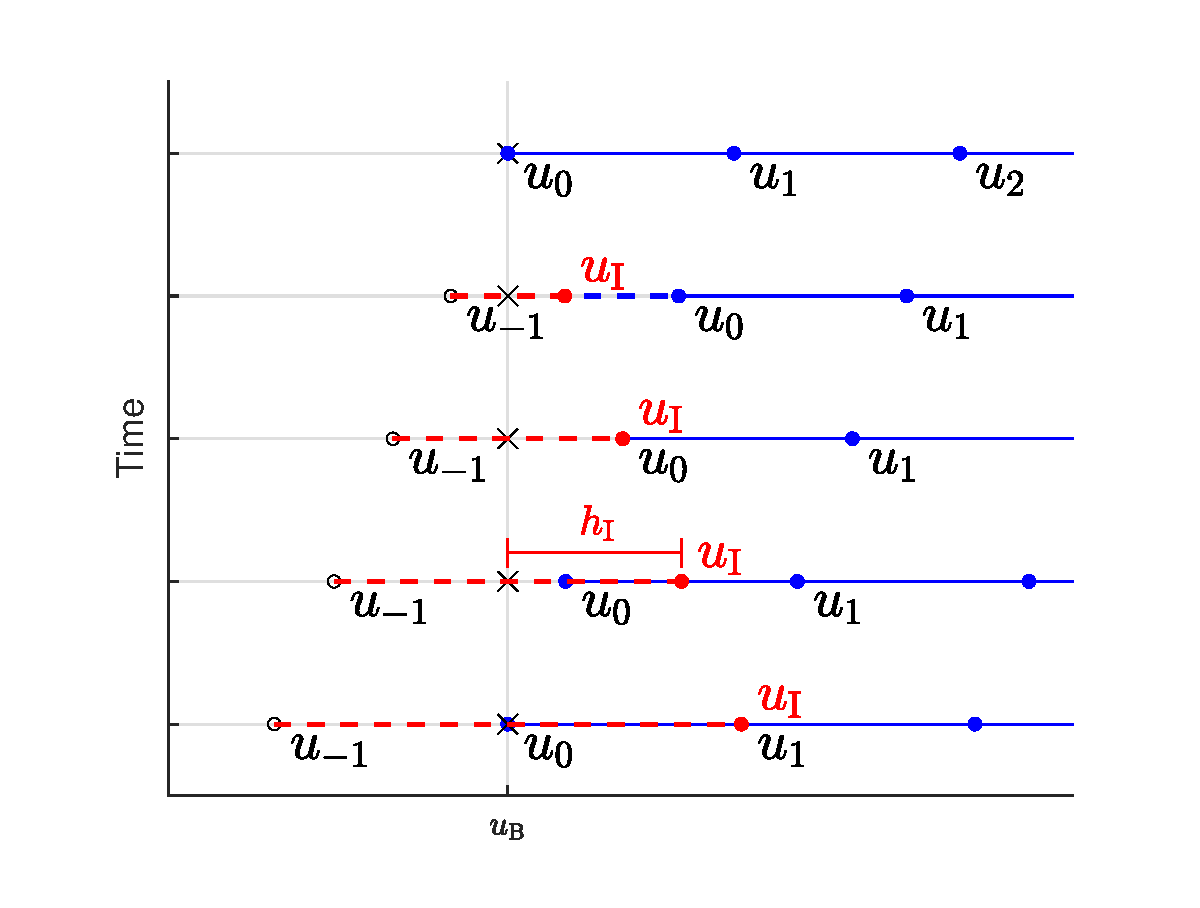
\includegraphics[width=0.6\columnwidth]{dynamicBoundaryDrawChange.eps}}
\caption{\label{fig:dynamicBoundary}{Boundary conditions at different values for $h$. Important to note is that the distance between $u_0$ and $u_{-1}$ always remains (the current) $h$. Then, from the location of $u_{-1}$, the location of $u_\text{I}$ (the interpolated point used to calculate the value of $u_{-1}$) is determined.}}
\end{figure}

% Using $\lambda = ck/h$, expanding \eqref{eq:1Dwave} at the boundary and applying \eqref{eq:expandedBoundCond}:
% \begin{equation}
%     \begin{aligned}
%         u_0^{n+1} &= 2u_0^n - u_0^{n-1} + \lambda^2 (u_1^n-2u_0^n + u_{-1}^n)\\
%         \xLeftrightarrow{\text{Eq. \eqref{eq:expandedBoundCond}}}\quad u_0^{n+1} &= 2u_0^n - u_0^{n-1} + \lambda^2 (u_1^n-2u_0^n - u_1^n)\\
%         u_0^{n+1} &= 2u_0^n - u_0^{n-1} - 2\lambda^2 u_0^n
%     \end{aligned}
% \end{equation}
% we can see that the virtual grid point $u_{-1}$ essentially cancels out the effect that $u_1$ has on $u_0$.  
% satisfy the boundary condition: the curvature around the boundary needs to be $0$. 

\section{Energy}
We can get the energy of Eq. \eqref{eq:1Dwave} by first taking the inner product with respect to $\delta_{t\cdot}u$ like
\begin{equation}
    \delta_{t+}\mathfrak{h} = \rho A\langle \delta_{t\cdot}u, \delta_{tt}u\rangle_\mathcal{D} - T \langle \delta_{t\cdot}u,\delta_{xx}u\rangle_\mathcal{D} = 0,
\end{equation}
using integration by parts to get
\begin{equation}\label{eq:innerProd}
    \delta_{t+}\mathfrak{h} = \rho A\langle \delta_{t\cdot}u, \delta_{tt}u\rangle_\mathcal{D} + T \langle \delta_{t\cdot}\delta_{x+}u,\delta_{x+}u\rangle_{\underline{\mathcal{D}}} = \mathfrak{b},
\end{equation}
where boundary term
\begin{equation}
    \mathfrak{b} = T (\delta_{t\cdot}u_N)(\delta_{x+}u_N) - T(\delta_{t\cdot}u_0)(\underbrace{\delta_{x+}u_{-1}}_{\delta_{x-}u_0})\ .
\end{equation}
Expanding Eq. \eqref{eq:innerProd} yields,
\begin{equation}
    \delta_{t+}\mathfrak{h} = \rho A \sum_\mathcal{D}h(\delta_{t\cdot}u)(\delta_{tt}u) + T \sum_{\underline{\mathcal{D}}}h(\delta_{t\cdot}\delta_{x+}u)(\delta_{x+}u)
\end{equation}
Then, using the following identities  
\begin{subequations}
\begin{align}
    (\delta_{t\cdot}u)(\delta_{tt}u) &= \delta_{t+}\left(\frac{1}{2}(\delta_{t-}u)^2\right) \quad \text{and}\label{eq:identity1}\\
    (\delta_{t\cdot}u)u &= \delta_{t+}\left(\frac{1}{2}u e_{t-}u\right)\label{eq:identity2}
\end{align}
\end{subequations}
we can finally obtain the energy $\mathfrak{h}$:
\begin{gather}
        \mathfrak{h} = \mathfrak{t} + \mathfrak{v}\quad \text{where}\\
    \mathfrak{t} = \frac{\rho A}{2} \sum_{\mathcal{D}} h (\delta_{t-}u_l^n)^2 \quad \text{and} \quad \mathfrak{v} =  \frac{T}{2}\sum_{\underline{\mathcal{D}}}h (\delta_{x+}u_l^n)(\delta_{x+}u_l^{n-1})
\end{gather}

In the case when $x_\text{I} \leq x_0$ (case \eqref{eq:xiSmaller}) we can find an energy definition for the left boundary:
\begin{equation}
    \begin{aligned}
        \delta_{t+}\mathfrak{h}_\text{l} &= T(\delta_{t\cdot}u_0)(\delta_{x-}u_0)\\
        &= \frac{T}{h}(\delta_{t\cdot}u_0)(u_0 - u_{-1})\\
        \xLeftrightarrow{u_{-1} = -\alpha u_0} \quad & = -\frac{T}{h}(\delta_{t\cdot}u_0)((1+\alpha)u_0)\\
        &
        = \frac{T(\alpha+1)}{h}(\delta_{t\cdot}u_0)u_0\\
        \xLeftrightarrow{\text{Eq. \eqref{eq:identity2}}} \quad & = \frac{T(1+\alpha)}{h}\delta_{t+}\left(\frac{1}{2}u_0^nu_0^{n-1}\right)\\
        \mathfrak{h}_l &= \frac{T(1+\alpha)}{2h}u_0^nu_0^{n-1}
    \end{aligned}
\end{equation}
The next step (after my vacation) will be to find the energy for case \eqref{eq:xiLarger} (if it exists....)
\bibliographystyle{plain}
\bibliography{bibliography}

\appendix
\section{Issue regarding increasing $T$}
If we decrease $T$, the points smoothly enter the scheme without issues. However, in the opposite case when we increase $T$ (moving from top to bottom in Figure \ref{fig:dynamicGrid}), the string will already be moving at $u_0$ and continue moving due to its inertia (the $\rho A \delta_{tt}u$ term). In other words, even though we can satisfy the $\delta_{xx}u_0 = 0$ part of the boundary condition, $u_0=0$ is harder to satisfy. Something needs to be figured out for this..

\end{document}
